%!TEX root = main.tex

\chapter{Modulation and Convolution}
\label{Modulation}


\begin{figure}[H]
	\begin{center}
		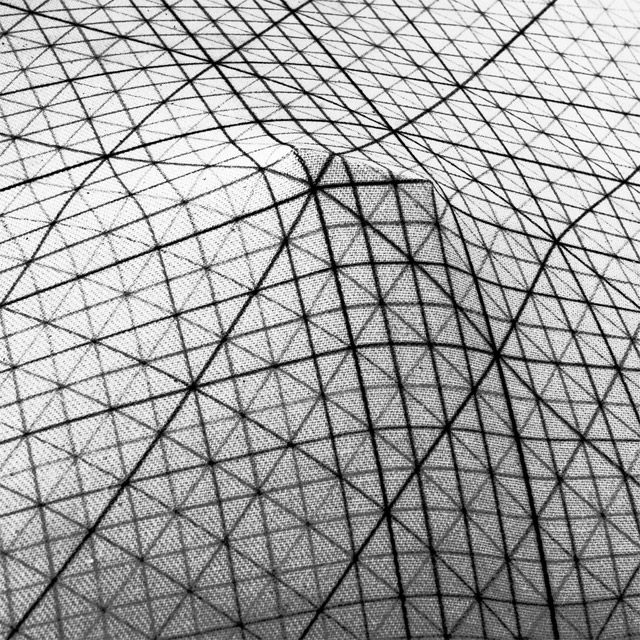
\includegraphics[width = 14cm]{img/surface-modulation_3.jpg}
		\caption{``Surface Modulation'' by Richard Sweeney}
		\label{fig:Surface Modulation}
	\end{center}
\end{figure}


\begin{center}
\begin{figure}[h!]
\tikzset{concept/.append style={fill={none}}}
\begin{tikzpicture}
  \path[mindmap,concept color=black,text=black]
    node[concept] {Modulation}
    [clockwise from=0]
    child[concept color=red!50!black] {
      node[concept] {AM}
      % }
      [clockwise from=90]
      child { node[concept] {Envelopes} }
      child { node[concept] {AM} }
      child { node[concept] {Ring Modulation} }
      % child { node[concept] {pro\-gramming languages} }
      % child { node[concept] {software engineer\-ing} }
    }  
    child[concept color=blue] {
      node[concept] (fm) {FM} 
      [clockwise from=-30]
    }
    child[concept color=red] { node[concept] (pm){Phase Modulation} }
    child[concept color=orange] { node[concept] (sd) {Sound design Challenge} };


\begin{pgfonlayer}{background}
    \draw [circle connection bar]
      (fm) edge (sd)
      (fm) edge (pm);
  \end{pgfonlayer}

\end{tikzpicture}
\caption{Lecture Contents}
\end{figure}
\end{center}


% \section{Notizen}

% kürzer. Modulation als sub einheit einplanen.
% Sounddesign challg. halbe stunde ok..

% Passt garnicht: (weil eher additive synth)
% https://www.youtube.com/watch?v=oKv9S6mxnXE


% Notation durchgehen.

% Aliasing besprochen?
% \href{https://www.youtube.com/watch?v=GBtHeR-hY9Y}{Water experiment}
% (youtube \glqq{}The Secret to Levitation\grqq{})

% AM, tremolo

% Envelopes in pd

% FM, vibrato

% sounddesign chall.

% Hü




\section{AM} % (fold)
\label{sub:AM}
In this section we will try amplitude modulation. Amplitude modulation is used for radio communication (so you'll need to understand this as a technician, modulation techniques are extremely important and this is maybe the simplest one) but also in sound design. We will try to understand the problem from different perspectives at once:
\begin{itemize}
	\item Doing some math
	\item listening to it
	\item brining it in context to beating waves
	\item seeing it as convolution in the frequency domain
\end{itemize}

Amplitude modulation means modulating the amplitude of a signal(surprise!). Modulating means changing over time by another signal. So we have some signal, say, a sine wave, and change its amplitude with another signal, say, another sine wave. Talking this concept and reducing it radically, we end up with figure \ref{fig:simpleAM}. 

\begin{figure}[H]
	\begin{center}
		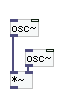
\includegraphics[width = 4cm]{img/ringNaive.png}
		\caption{Simplest form of ``Ring modulation''.}
		\label{fig:simpleAM}
	\end{center}
\end{figure}
Of course, we get no sound in figure \ref{fig:simpleAM} because the frequencies are not initialized, but it shows the general principle. The caption of that figure says ``Ring Modulation''. Let's quickly get some vocabulary straight:\\
\begin{itemize}
	\item ``Amplitude modulation'' might mean any modulation of amplitude
	\item ``Ring Modulation'' means \textit{bi-polar} amplitude modulation.
	\item In sound design, ``Amplitude Modulation'' might specifically mean unipolar amplitude modulation.
\end{itemize}

And some more vocabulary to put what we are doing in a musical context:
\begin{itemize}
	\item Modulating the amplitude is called ``Tremolo'' in music \footnote{sadly, the fender stratocaster's ``Tremolo Arm'' is used to control the pitch. Ignore Fender, they got it wrong. You can trust that most guitar players are confused because of this.}
	\item Modulating the pitch or frequency (``FM'') is called ``vibrato'' in a musical context.\footnote{Maybe think about it like this: The F in FM is a bit like the v in vibrato. Just to avoid confusion..}
\end{itemize}

Enough words, let's look at what AM looks like, look at figure \ref{fig:AMViz}.


\begin{figure}[h!]
	\centering
	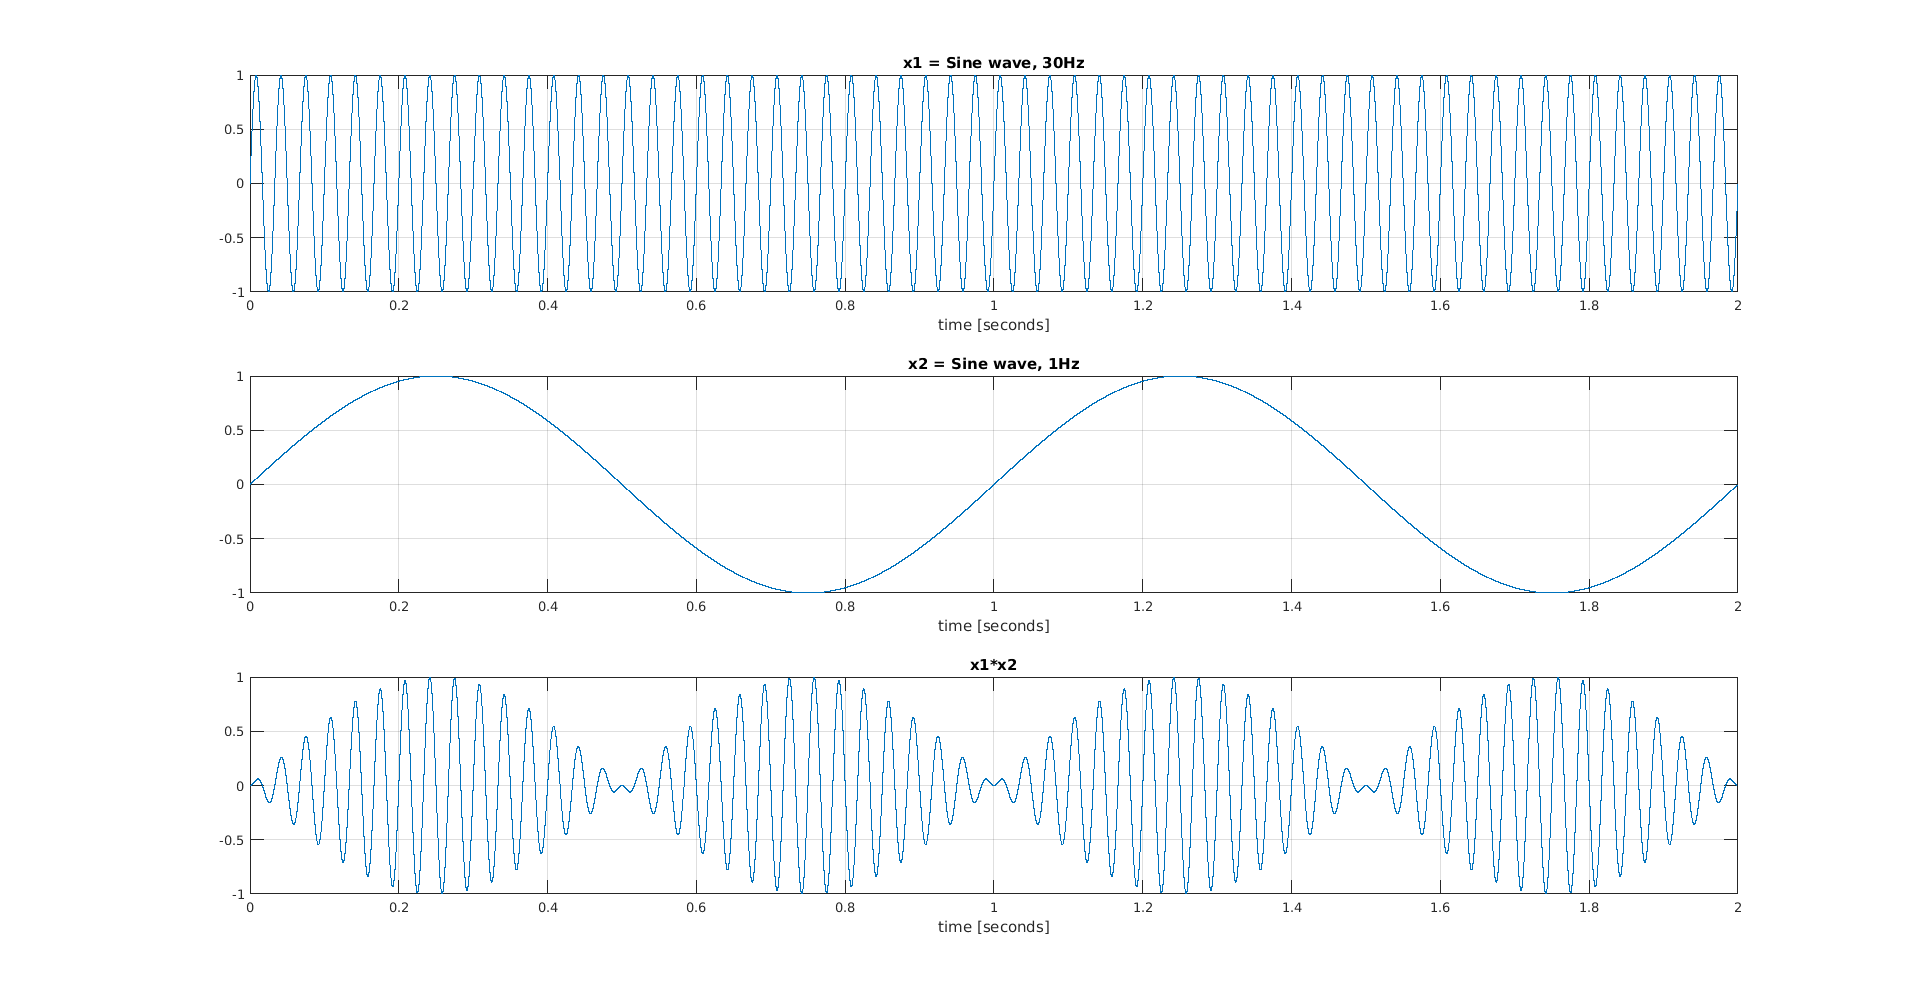
\includegraphics[width=\textwidth]{AMviz.png}
	\caption[AM time domain]
	{Looking at AM in the time domain}
	\label{fig:AMViz}
\end{figure}


\begin{question}
	If we would listen to the signal depicted in the bottom plot of figure \ref{fig:AMViz}, what do you think we would hear? Try to imagine! If you can't, use pure data to test it! That's why we are using pd.
\end{question}
\begin{Answer}
	We would hear a 30Hz sine wave repeatedly rising and falling in amplitude.
\end{Answer}



\begin{question}
	Next question, same plot, same signal. So hopefully you found out that we hear a 30 Hz sine with rising and falling amplitude. At what frequency does the amplitude rise and fall? Remember we are modulating with a 1 Hz sine.
\end{question}
\begin{Answer}
	Two Hertz. 
\end{Answer}

Maybe you remember from the waveshaping chapter that we actually calculated what frequencies should come out of AM. Also maybe you remember that sum and difference frequencies should come out, but here we still hear the 30 Hz, just getting louder and softer, so what's wrong? Let's look at the formulas again, just for reference:
\begin{equation}
	cos(a)\cdot cos(b) = \frac{cos(a+b) + cos(a-b)}{2}
\end{equation}

So, let's calculate this. We have two oscillators, $x_1(t) = cos(30t2\pi)$ and $x_2(t)=cos(t2\pi)$. We multiply them, ending up with:

\begin{equation}
	y(t) = cos(30t2\pi) \cdot cos(t2\pi)
\end{equation}
Ok, the above formula tells us this means:
\begin{equation}
	y(t) = \frac{cos(30t2\pi+t2\pi)+cos(30t2\pi-t2\pi)}{2}
\end{equation}
We can now simplify to:
\begin{equation}
	y(t) = \frac{cos((30+1)t2\pi)+cos((30-1)t2\pi)}{2} = \frac{cos(31t2\pi)+cos(29t2\pi)}{2}
\end{equation}

Hm, so we get out a 31Hz and 29Hz oscillator. What about that rising and falling in amplitude that we hear \textit{and} observe in the plot, surely there must be something wrong! Do you have a solution to this?\\

Let's use pure data to help us understand. Make two oscillators, one with 29Hz and one with 30Hz, what do you hear?

\begin{figure}[h!]
	\centering
	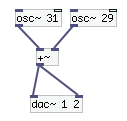
\includegraphics[width=5cm]{beating.png}
	\caption[adding two oscillators]
	{Adding two oscillators with frequencies very close to each other}
	\label{fig:beating}
\end{figure}

If you listen to what is depicted in figure \ref{fig:beating}, you will in fact hear the same as if you do the 30Hz /1 Hz amplitude modulation (which indicates that our formula above is correct). What we hear is a phenomenon called beating. The phase of the two oscillators is canceling each other out at regular intervals because the frequencies are so close to each other. In fact the frequency of the beating $f_{beat}$ is always 
\begin{equation}
	f{beat}=|f_1-f_2|
\end{equation}
So the difference of the two frequencies.



\begin{figure}[H]
	\begin{center}
		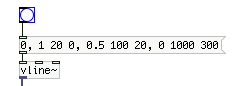
\includegraphics[width = 14cm]{img/simpleEnv.png}
		\caption{caption}
		\label{fig:name}
	\end{center}
\end{figure}

\textbf{Multiplying two signals in the time domain is equvalent to convolution in the frequency domain and vice versa.
}


Amplitude Modulation. \glqq{}tremolo\grqq{}

Ringmodulation = Bipolar,
AM = Unipolar

\section{FM} % (fold)
\label{sub:FM}
\comm{Work in progress}
Frequency Modulation. \glqq{}Vibrato\grqq{}


\begin{figure}[H]
	\begin{center}
		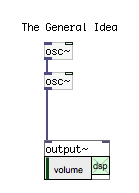
\includegraphics[width = 7cm]{img/FMgeneral.png}
		\caption{The General Idea of FM}
		\label{fig:fmIdea}
	\end{center}
\end{figure}

Naive parameters are ${f_c}$ (Carrier Frequency), ${f_m}$ (Modulator Frequency), and ${A_m}$ (modulation Amount).

\begin{figure}[H]
	\begin{center}
		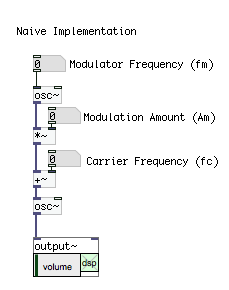
\includegraphics[width = 10cm]{img/FMnaive.png}
		\caption{Naive Implementation with Direct Parametrization.}
		\label{fig:fmNaive}
	\end{center}
\end{figure}

The output frequencies will be
\begin{equation}
	f_c \pm n \cdot f_m
\end{equation}

Typically, FM is controlled via \textit{Index}, \textit{Ratio}, and fundamental Frequency. The Index, ${I}$ is given by Modulation Depth and Modulator Frequency.

\begin{equation}
I = \frac{A_m}{f_m}
\end{equation}

A more controllable Implementation will generate the naive parameters from a Ratio, ${R}$, the Carrier Frequency and the Index:
\begin{equation}
	f_m = \frac{f_c}{R}
\end{equation}

\begin{equation}
	A_m = \frac{I}{f_m}
\end{equation}

\begin{figure}[H]
	\begin{center}
		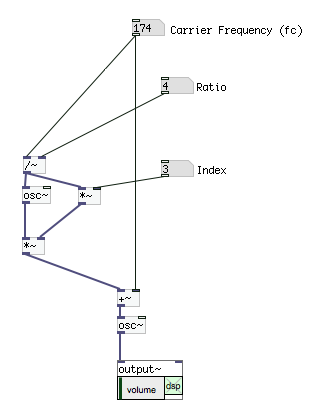
\includegraphics[width = 14cm]{img/FMcorrect.png}
		\caption{FM with Index and Ratio}
		\label{fig:fmComplete}
	\end{center}
\end{figure}

\section{Hausübung}
\label{sub:Hausuebung}
Andy Farnell, \href{http://aspress.co.uk/ds/pdf/pd_intro.pdf}{pd intro} chapter 6, lesen
